% article example for classicthesis.sty
\documentclass[10pt,a4paper]{article} % KOMA-Script article scrartcl
\usepackage{import}
\usepackage{xifthen}
\usepackage{pdfpages}
\usepackage{transparent}
\newcommand{\incfig}[1]{%
    \def\svgwidth{\columnwidth}
    \import{./figures/}{#1.pdf_tex}
}
\usepackage{lipsum}     %lorem ipsum text
\usepackage{titlesec}   %Section settings
\usepackage{titling}    %Title settings
\usepackage[margin=10em]{geometry}  %Adjusting margins
\usepackage{setspace}
\usepackage{listings}
\usepackage{amsmath}    %Display equations options
\usepackage{amssymb}    %More symbols
\usepackage{xcolor}     %Color settings
\usepackage{pagecolor}
\usepackage{mdframed}
\usepackage[spanish]{babel}
\usepackage[utf8]{inputenc}
\usepackage{longtable}
\usepackage{multicol}
\usepackage{graphicx}
\graphicspath{ {./Images/} }
\setlength{\columnsep}{1cm}

% ====| color de la pagina y del fondo |==== %
\pagecolor{black}
\color{white}



\begin{document}
    %========================{TITLE}====================%
    \title{{  9th Laboratory: Malware as service  }}
    \author{{Rodrigo Castillo}}
    \date{\today}

    \maketitle


     % ====| Loguito |==== %
    
\includegraphics[width=0.1\linewidth]{negro_cara.png}
    %=======================NOTES GOES HERE===================%

    \section{Q: Read section "Malware Behavior" and describe the difference
    between Dowloaders, Launchers and Backdoors?}
        \begin{itemize}
            \item {\textbf{Downloader}  A downloader is a program with the
                capability of \textbf{download} other programs into the
                victim's machine}
            \item {\textbf{Launcher}  a launcher is a program with the
                capability of \textbf{launch} processes into the victim's
            machine}
            \item {\textbf{Backdoor}  a backdoor is a program or a
                vulnerability that lets the atacker spawn a reverse shell into
                the victim's machine whenever he wants}
        \end{itemize}

        However those definitions are just definitions to clasify malware,
        somethimes, malware can be placed in more than 1 category.


    \newpage
    \section{Q: Read the section "Reverse Shell". Then, create and test a
    Reverse shell using the following commands.}

        \begin{figure}[h!]
            \centering
            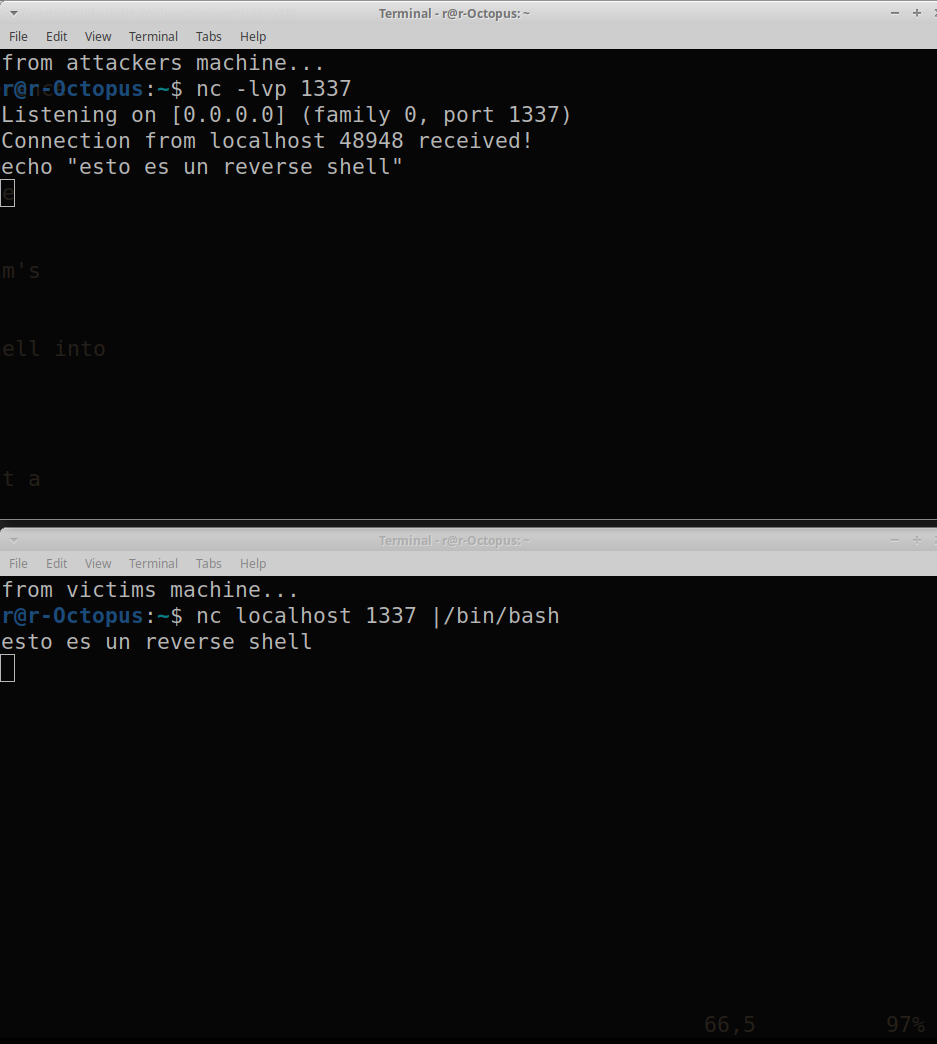
\includegraphics[width=0.6\linewidth]{reverse.png}
            \caption{reverse shell}
            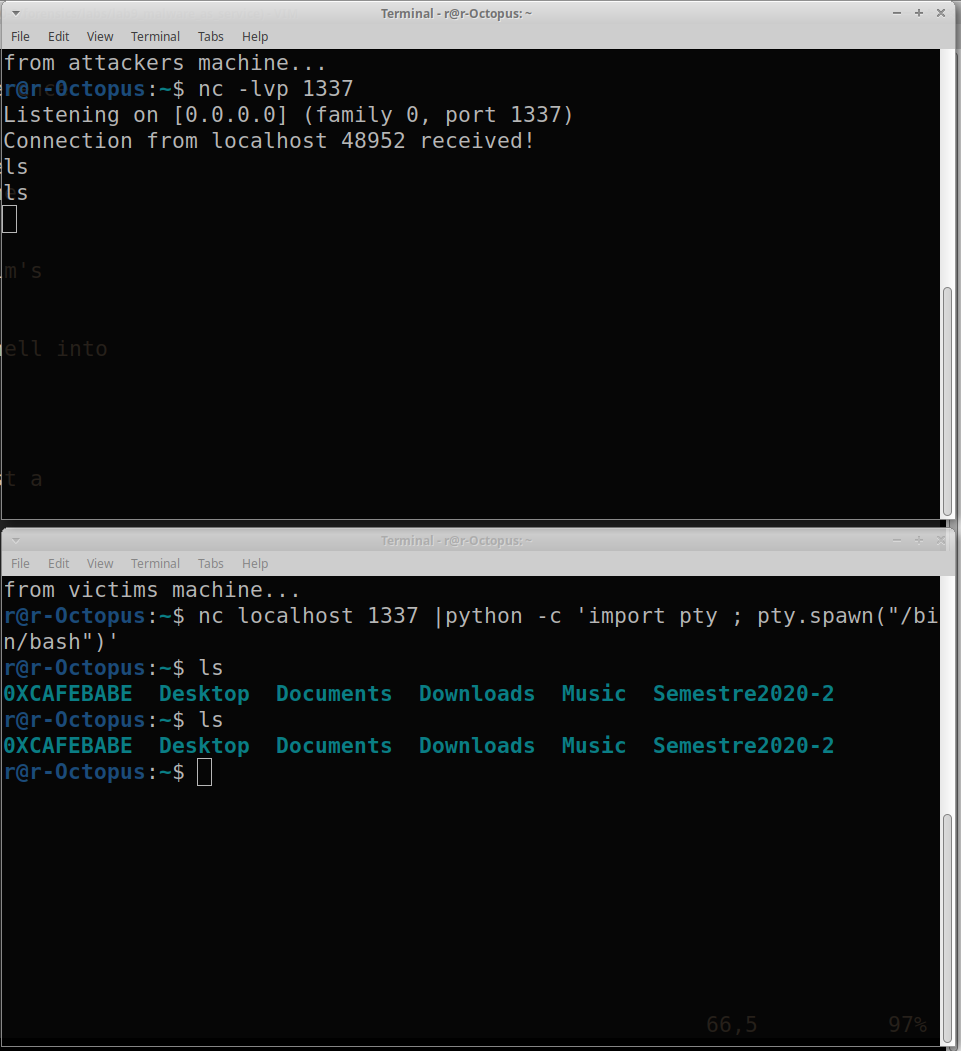
\includegraphics[width=0.6\linewidth]{global_reverse_shell.png}
            \caption{reverse shell using pty library python}
            \label{fig}
        \end{figure}











    %=======================NOTES ENDS HERE===================%

    % bib stuff
    \nocite{*}
    \addtocontents{toc}{{}}
    \addcontentsline{toc}{section}{\refname}
    \bibliographystyle{plain}
    \bibliography{../Bibliography}
\end{document}
